\RequirePackage{plautopatch}

\documentclass[a4paper, 10pt]{ltjsarticle}


% マージン設定
\usepackage[top=20mm, bottom=20mm, left=20mm, right=20mm]{geometry}

% LuaLaTeX用日本語対応パッケージ
\usepackage{luatexja}
\usepackage{luatexja-fontspec}

% 必要なパッケージ
\usepackage{fontspec}
\usepackage{titlesec}
\usepackage{graphicx}
\usepackage{amsmath}
\usepackage{amssymb}
\usepackage{hyperref}
\usepackage[english, japanese]{babel}
\usepackage{indentfirst}
\usepackage{tikz} % カスタム点線用
\usepackage{authblk} % 著者・所属パッケージ
\usepackage{here}
\usepackage{caption}
\usepackage{bookmark}

\begin{document}

\thispagestyle{empty}
\begin{center}

\vspace{20mm}
{\Large\noindent 2020年度 卒業(修士)論文}\\
\vspace{40mm}
{\huge\noindent\textbf{論文タイトル}}\\
\medskip
{\huge\noindent\textbf{論文タイトル(2行目)}}\\
\vspace{\baselineskip}
{\huge\noindent\textbf{英語title}}\\
\medskip
{\huge\noindent\textbf{英語title(2行目)}}\\
\vspace{40mm}

{\Large\noindent
2021年1月31日\\
\vspace{\baselineskip}
指導教員 ◯◯◯◯    \\
\vspace{\baselineskip}
◯◯◯大学\\
所属 \\
\vspace{\baselineskip}
学籍番号 名前\\
name \\
}
\vspace{40mm}

\end{center}

\thispagestyle{empty}
\clearpage
\subsection{アドホックネットワークの技術的課題}
\subsubsection{隠れ端末問題}
隠れ端末問題とは、図1のようにノードAとCがノードBに対して通信を行うとき、ノードAとCはお互いの存在が隠れてしまい、
現在誰も通信を行なってないと思い込んで同時にノードBへと通信を行いデータが衝突してし壊れてしまう問題である。%
\begin{figure}[H]
  \centering
  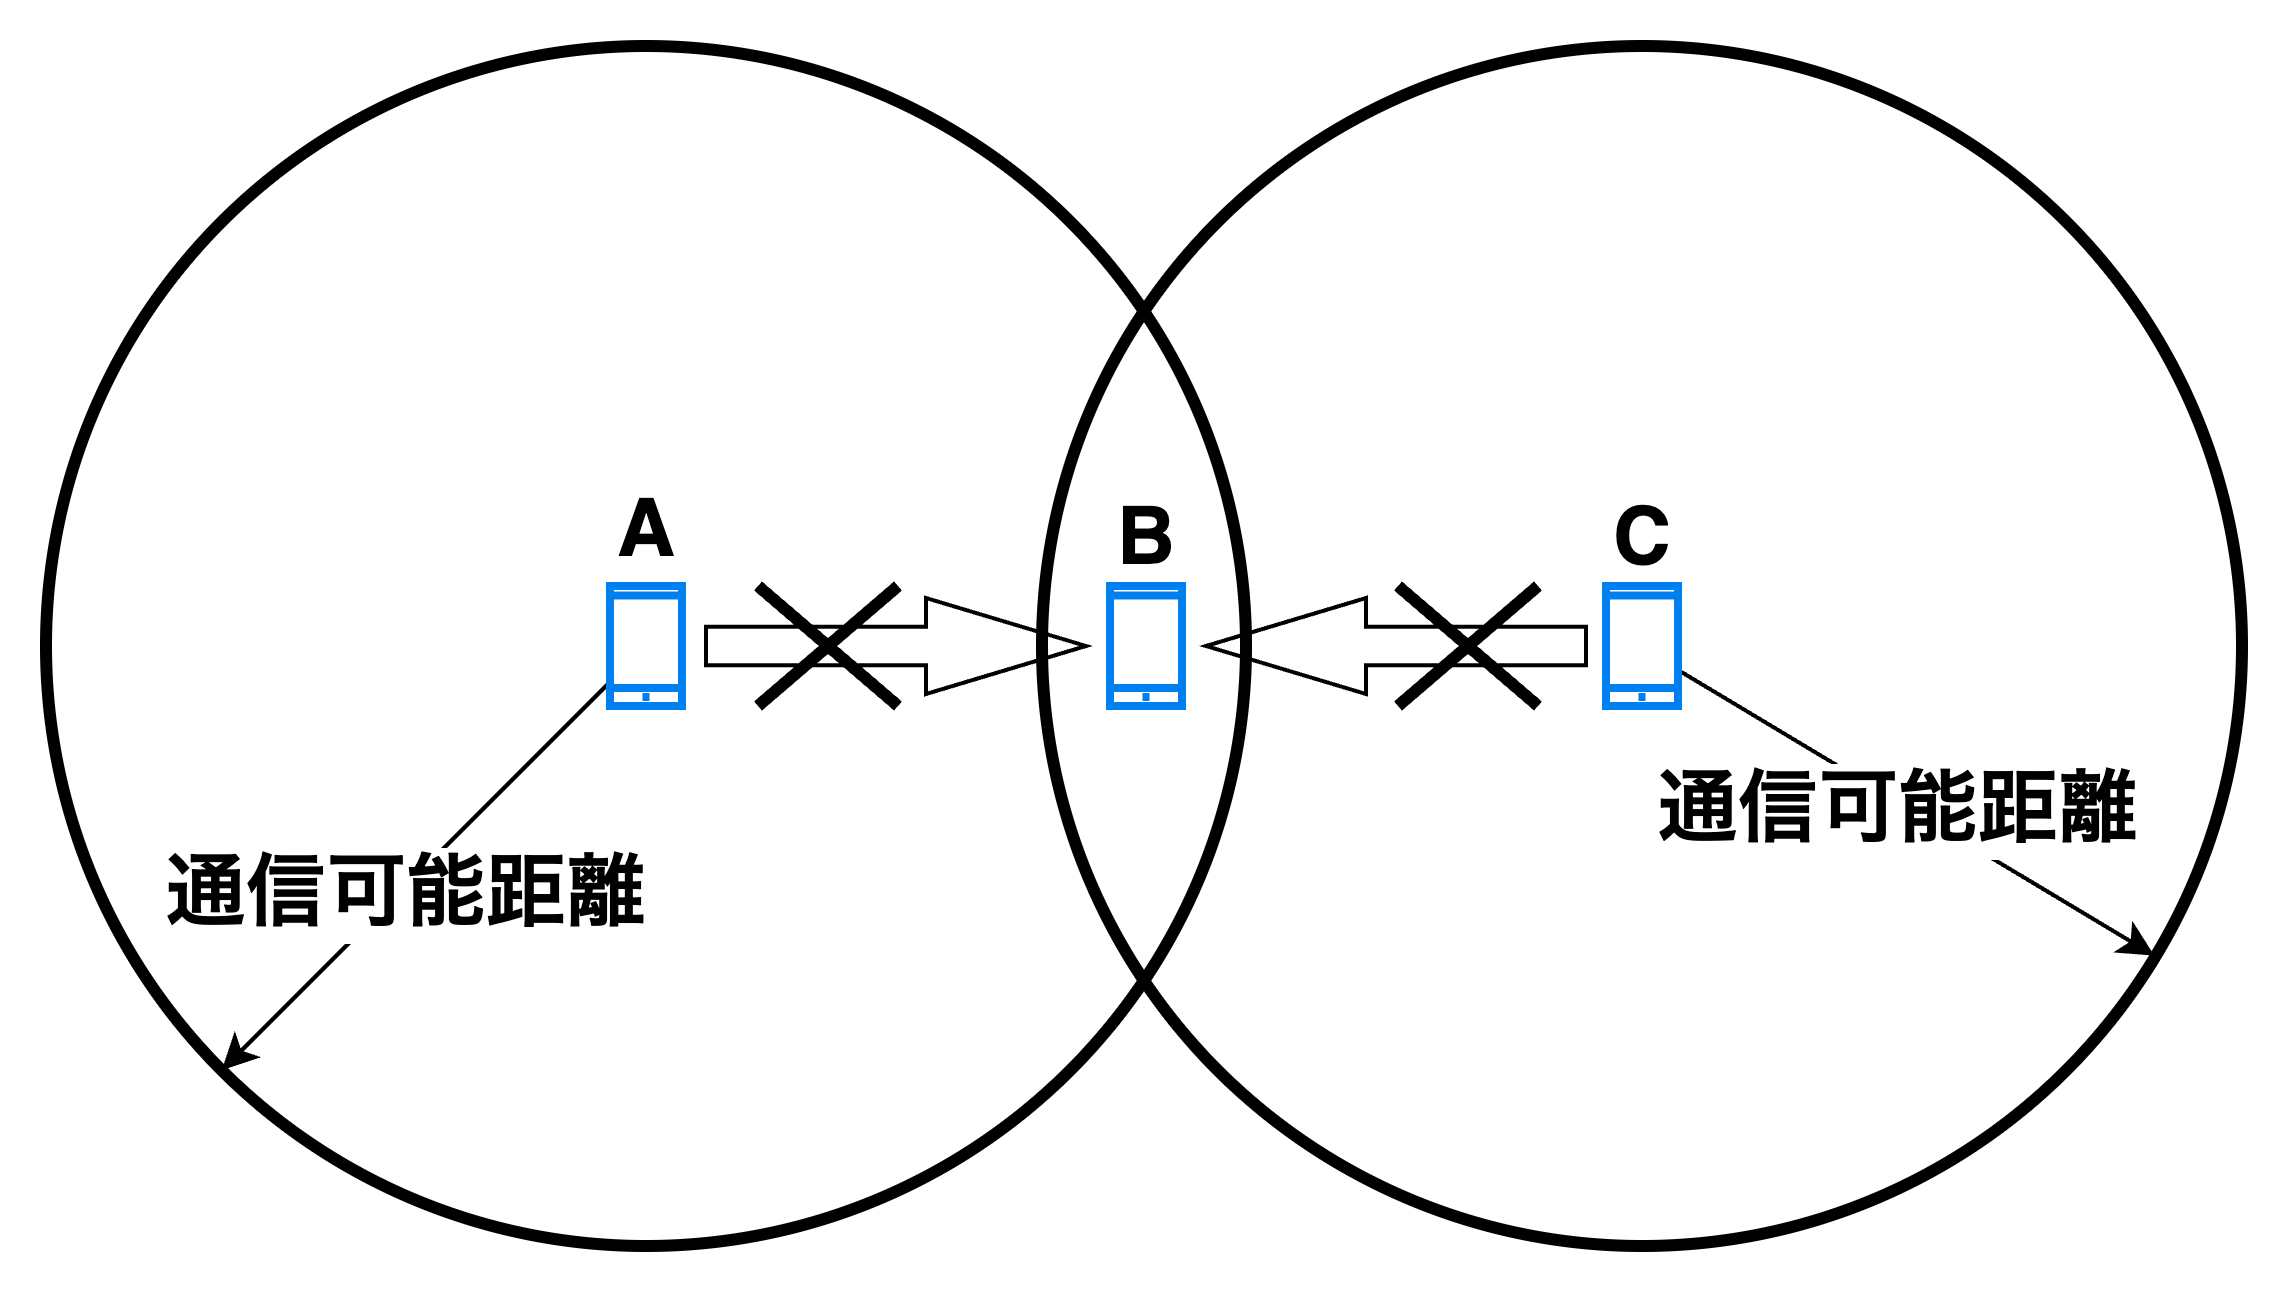
\includegraphics[width=70mm]{hidden_terminal_problem.png}
  \caption{隠れ端末問題}
\end{figure}

\subsubsection{さらし端末問題}
さらし端末問題とは、図2のようにノードAがDと通信を行なっているときノードBは端末Cと通信ができそうだが、
ノードAがDと通信を行なっているため周辺にいる他ノードは通信の抑制がされてしまい、
伝送速度や通信品質の低下が発生してしまう問題である。%
\begin{figure}[H]
  \centering
  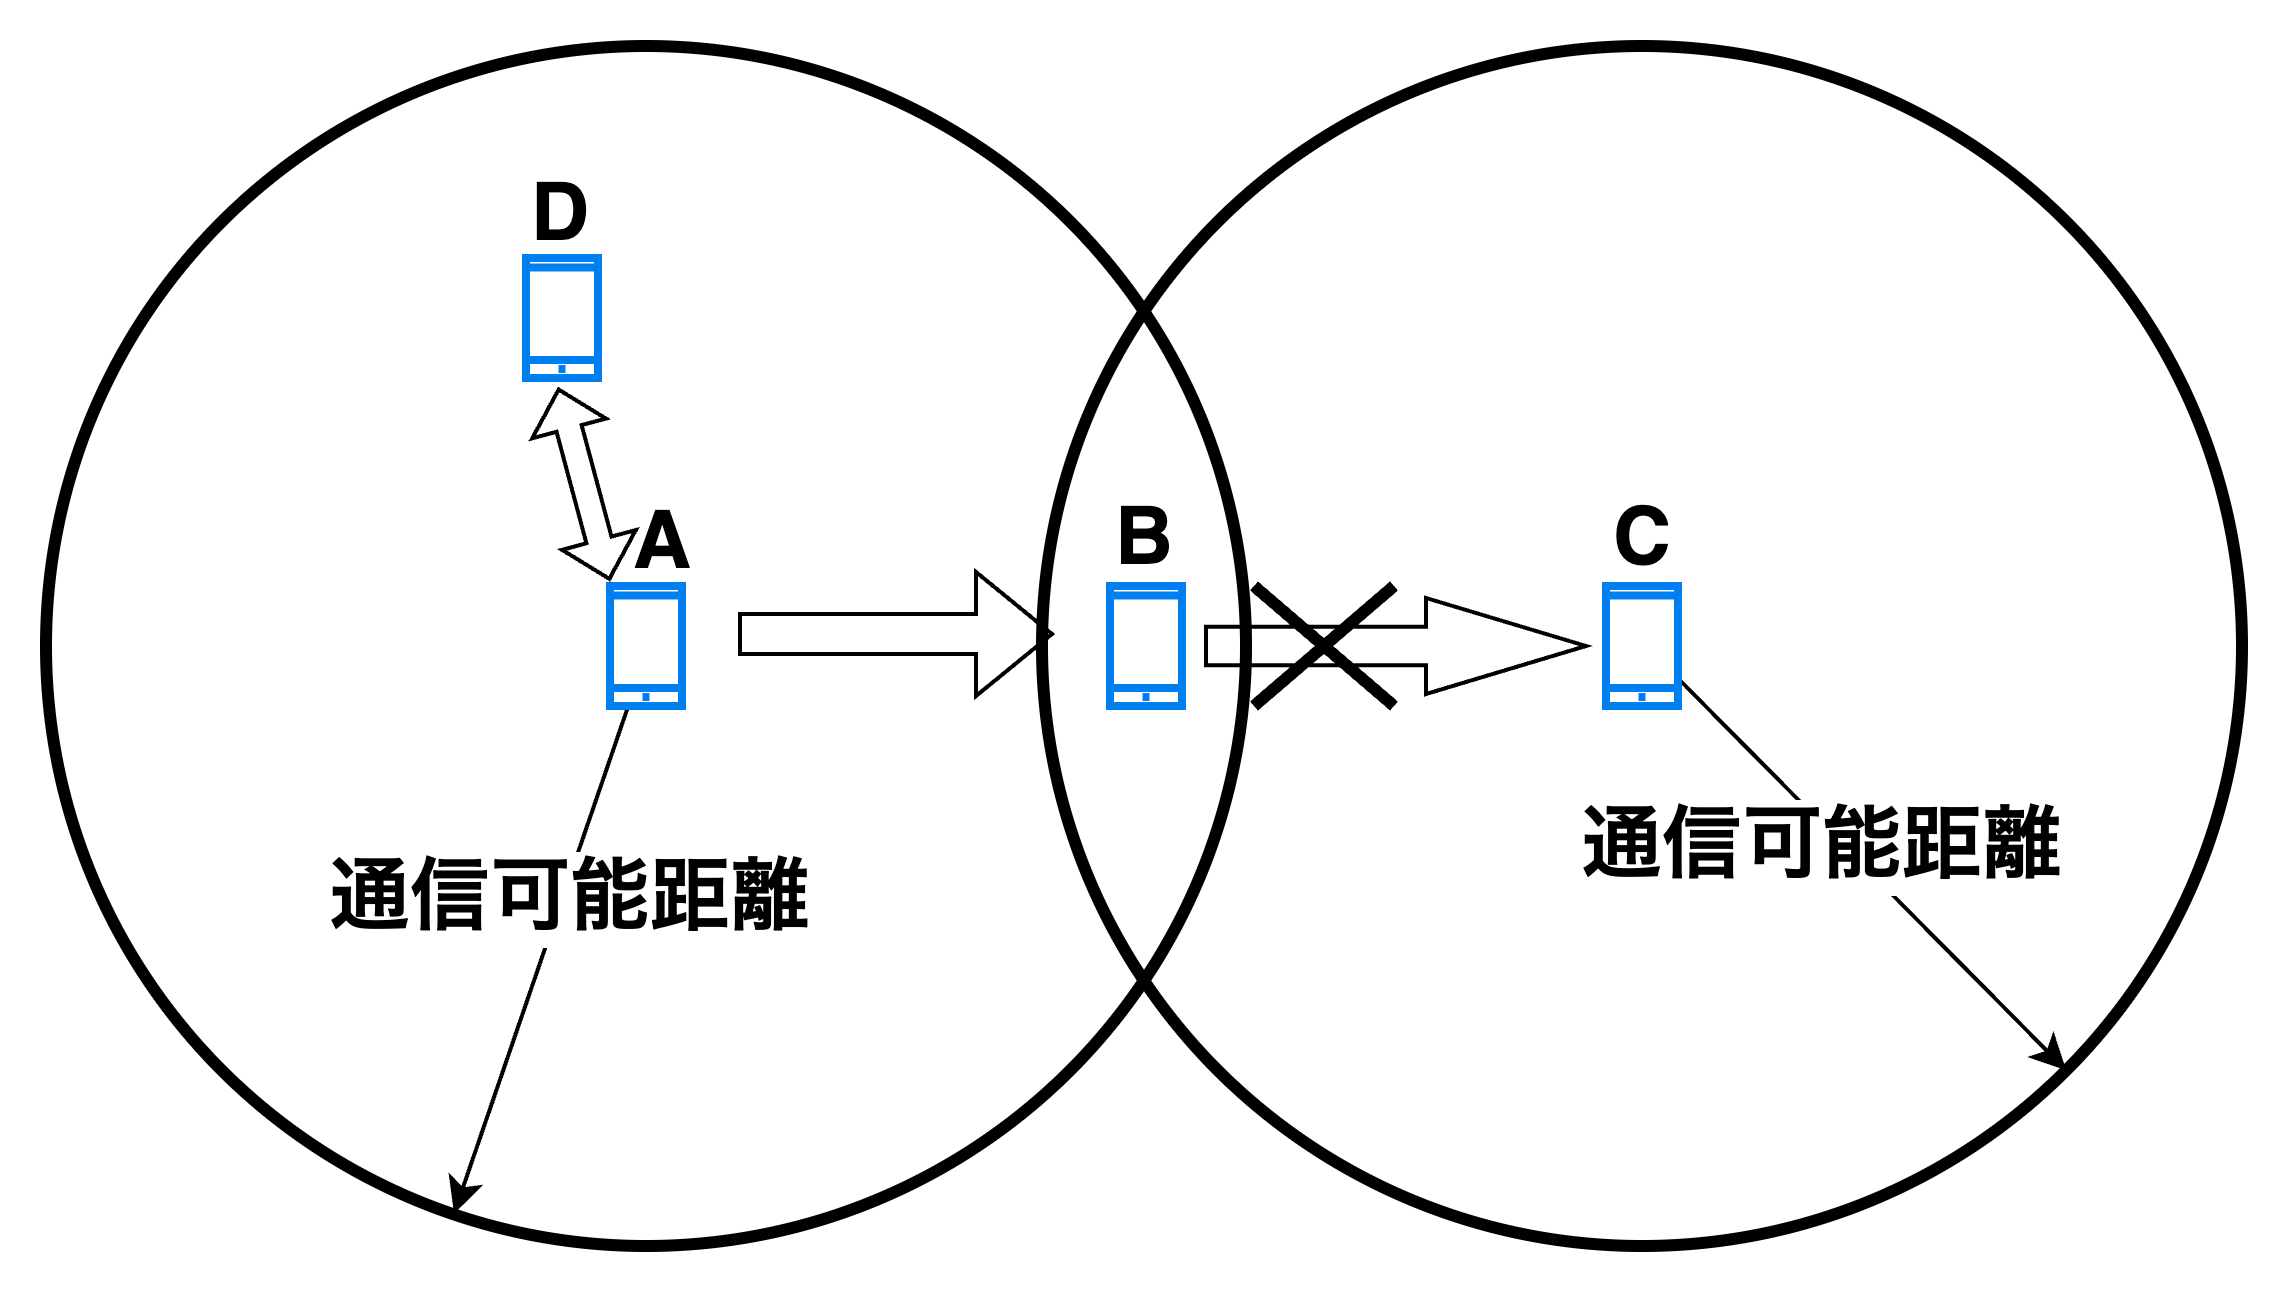
\includegraphics[width=70mm]{exposed_terminal_problem.png}
  \caption{さらし端末問題}
\end{figure}
\end{document}